\documentclass[12pt,a4paper]{article}
\usepackage[latin1]{inputenc}
\usepackage{amsmath}
\usepackage{amsfonts}
\usepackage{amssymb}
\usepackage{graphicx}
\usepackage{hyperref}
\usepackage{textcomp}
\usepackage{listings}

\author{}
\date{}
\title{
	\setlength\parskip{\baselineskip}
	
\includegraphics[width=0.7\linewidth]{../logo.png}
	\label{fig:MyoMapper}\\ \ \\ \ \\ \  \\ \ \\ \ \\
	DOCUMENTATION 
	}

\begin{document}
	
\maketitle
\thispagestyle{empty}	
\newpage
\tableofcontents
\thispagestyle{empty}	
\newpage

\setlength\parskip{\baselineskip}

\section*{Acknowledgements}
Myo Mapper is a software developed by Balandino Di Donato and supported by \href{http://integra.io/}{Integra Lab} , \href{http://www.bcu.ac.uk/conservatoire}{Birmingham Conservatoire}, and \href{http://www.bcu.ac.uk/}{Birmingham City University}.


\includegraphics[height=0.065\linewidth]{../integra} 
\includegraphics[height=0.065\linewidth]{../cons}

\section*{License}
\textcopyright Balandino Di Donato - 2016

Permission is hereby granted, free of charge, to any person obtaining a copy of this software and associated documentation files (the "Software"), to deal in the Software without restriction, including without limitation the rights to use, copy, modify, merge, publish, distribute, sublicense, and/or sell copies of the Software, and to permit persons to whom the Software is furnished to do so, subject to the following conditions:

The above copyright notice and this permission notice shall be included in all copies or substantial portions of the Software.


THE SOFTWARE IS PROVIDED "AS IS", WITHOUT WARRANTY OF ANY KIND, EXPRESS OR IMPLIED, INCLUDING BUT NOT LIMITED TO THE WARRANTIES OF MERCHANTABILITY, FITNESS FOR A PARTICULAR PURPOSE AND NONINFRINGEMENT. IN NO EVENT SHALL THE AUTHORS OR COPYRIGHT HOLDERS BE LIABLE FOR ANY CLAIM, DAMAGES OR OTHER LIABILITY, WHETHER IN AN ACTION OF CONTRACT, TORT OR OTHERWISE, ARISING FROM, OUT OF OR IN CONNECTION WITH THE SOFTWARE OR THE USE OR OTHER DEALINGS IN THE SOFTWARE.

\newpage
\section{Introduction}
Myo Mapper is an open source application to map Thalmic Labs's Myo armband\footnote{The Thalmic Labs's Myo armband is a wearable gesture control and motion control device that lets you take control of your phone, computer, and so much more, touch-free. Find out more here: \url{https://www.myo.com/}.} into OSC\footnote{Open Sound Control (OSC) is a protocol for communication among computers, sound synthesizers, and other multimedia devices that is optimized for modern networking technology. Find out more, \url{http://opensoundcontrol.org/introduction-osc}} and MIDI\footnote{MIDI is an industry standard music technology protocol that connects products from many different companies including digital musical instruments, computers, tablets and smartphones. \url{https://www.midi.org/}} parameters. Myo Mapper can be downloaded here \url{http://www.balandinodidonato.com/myomapper/} and its source code here: \url{https://github.com/balandinodidonato/MyoMapper}.

	\begin{figure}[h]
		\centering
		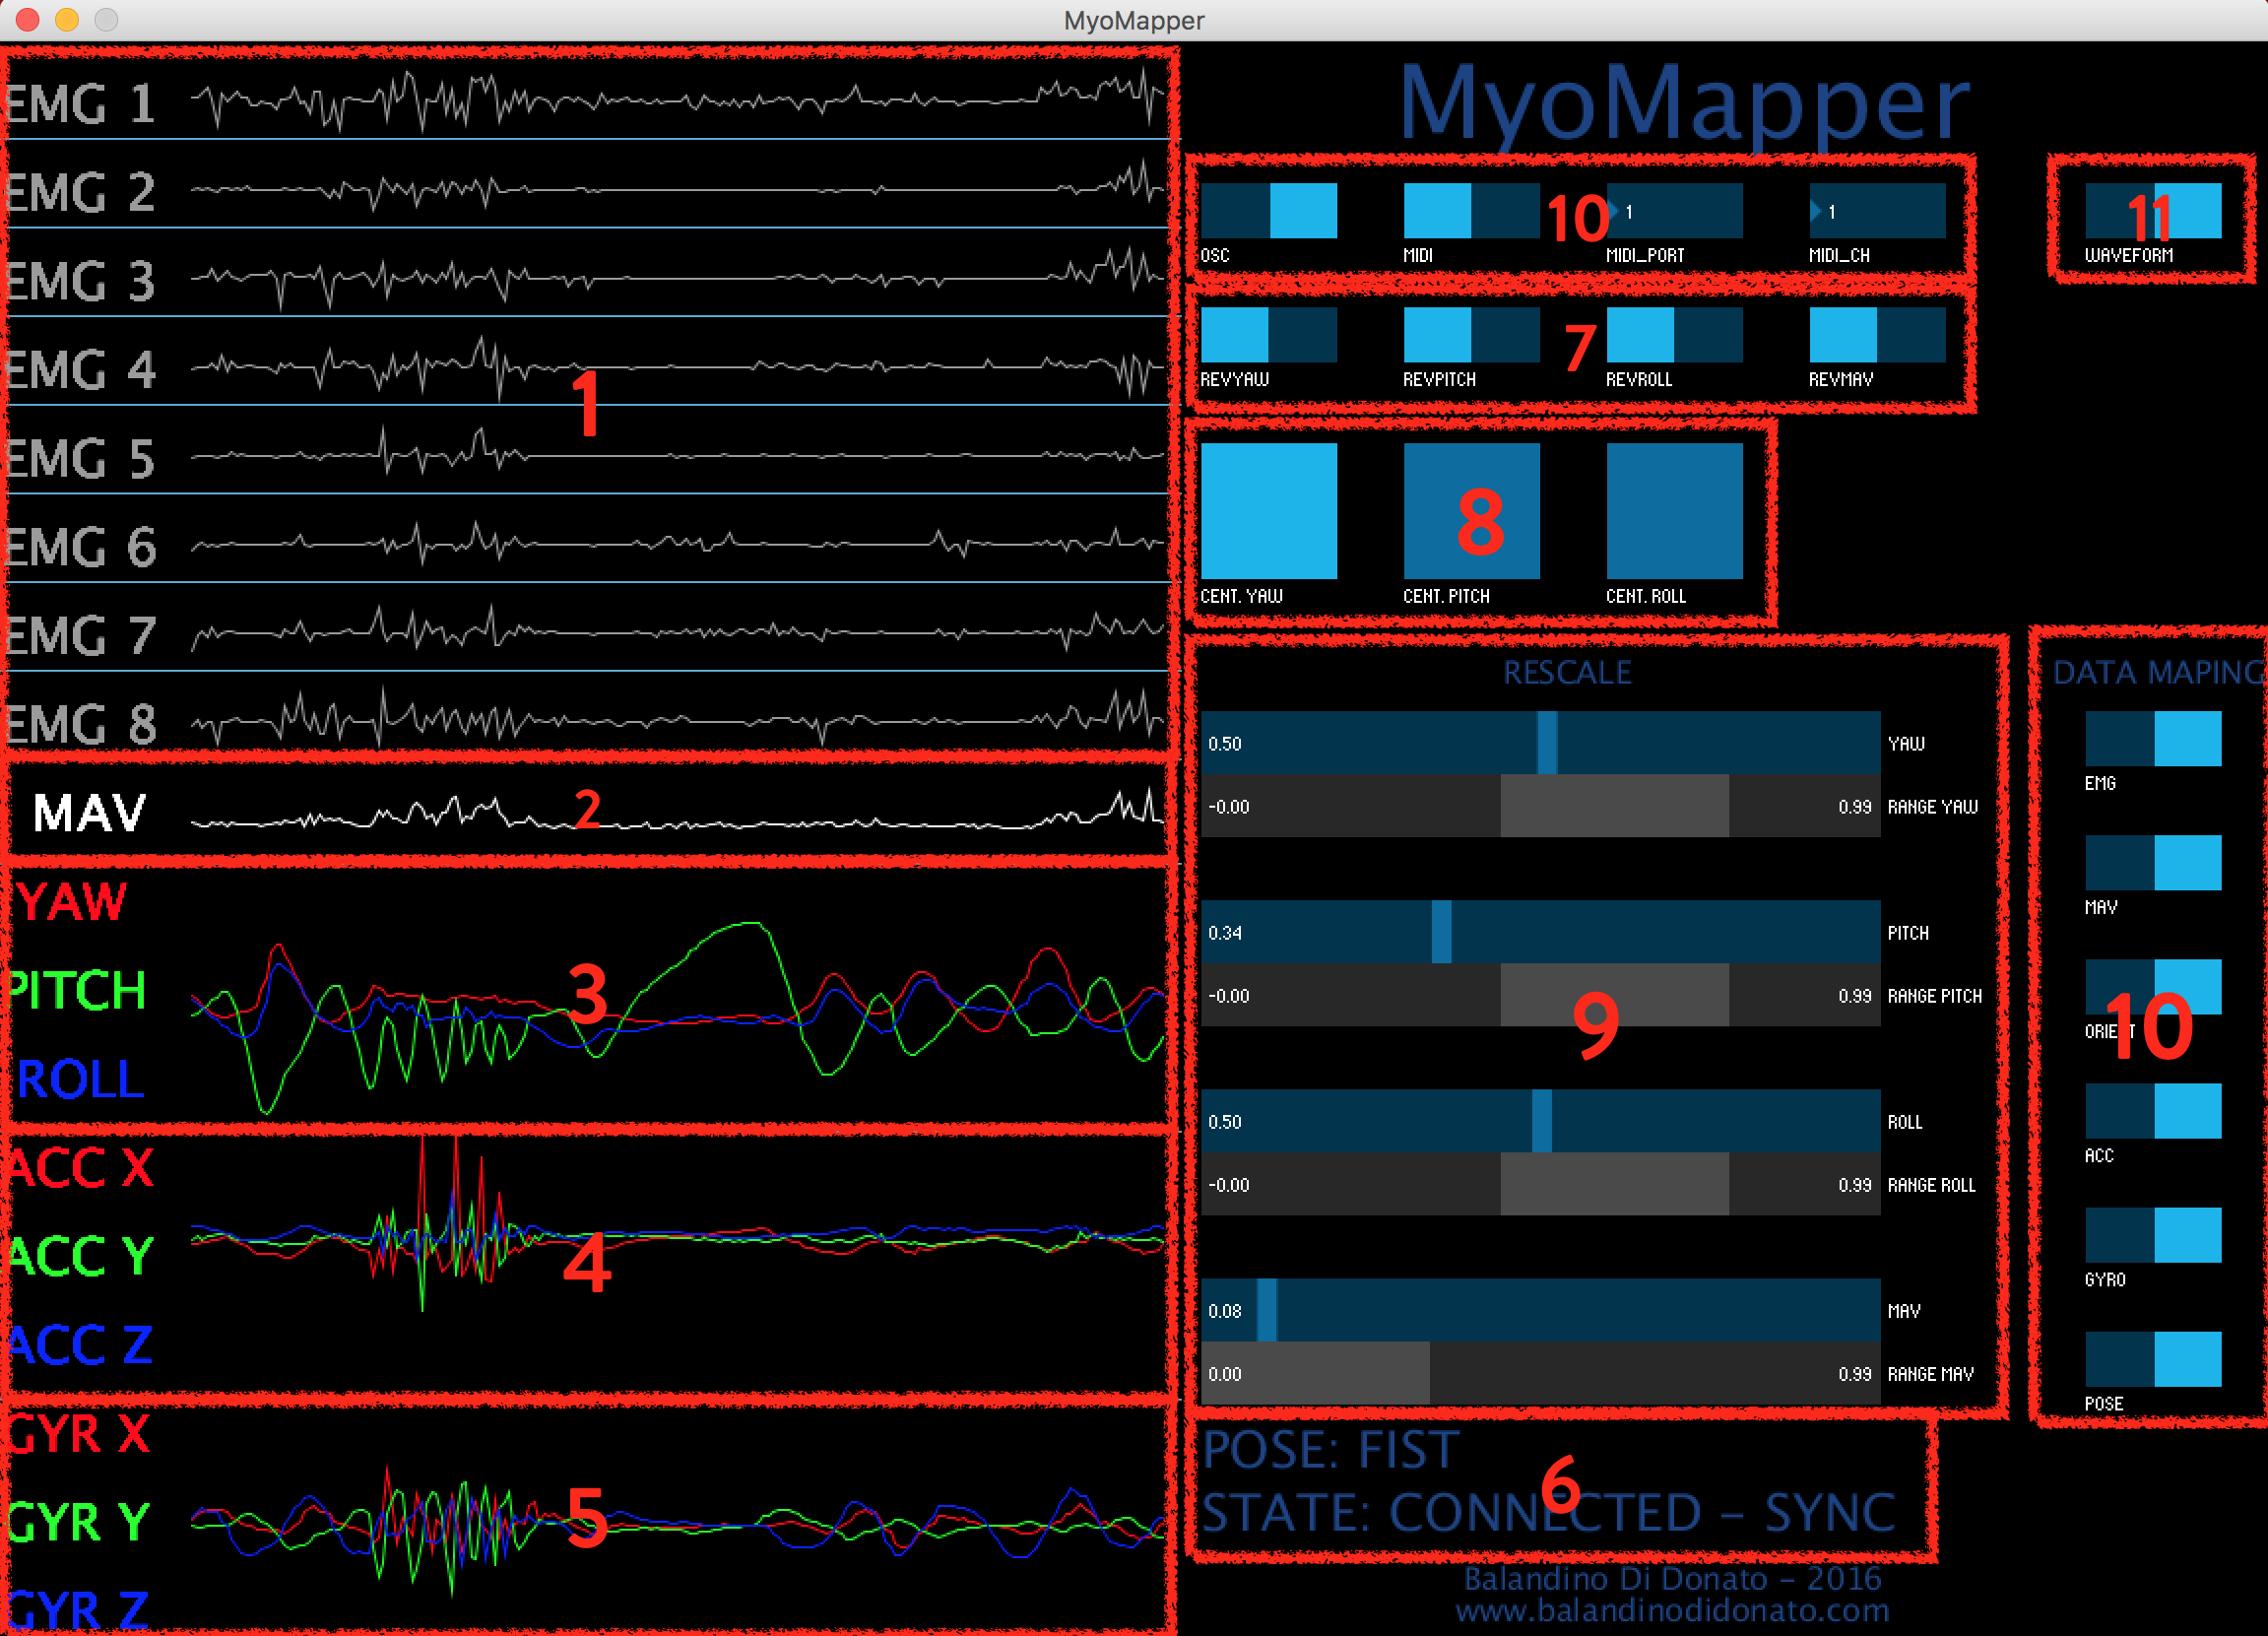
\includegraphics[width=1\linewidth]{../MyoMapper}
		\caption{MyoMapper screenshot}
		\label{fig:MyoMapperIntro}
	\end{figure}

\newpage

\section{Install Myo Mapper}
To get Myo Mapper working you have to follow just few steps listed below.

\begin{itemize}
	\item Download Myo Connect for Windows or Mac\footnote{Myo Connect, \url{https://developer.thalmic.com/downloads}}.
	\item Launch Myo Connect
	\item Install the unlock.myo connector.
	\item Open the Application Manager
	\subitem - +Add 
	\subitem - \textless MyoMapper folder\textgreater \textfractionsolidus unlock.myo
	\item It is not mandatory, yet it is better if you disable off all others scrips.
	\item Connect your Myo armband from the Armband Manager
	\item Verify Myo Connect detect your gestures
	\item Launch Myo Mapper
\end{itemize}

For more support about adding new connectors please visit the Myo support page\footnote{Adding new connectors, \url{https://support.getmyo.com/hc/en-us/articles/204156049-Adding-new-Connectors}}.

\newpage

\section{GUI}

	Myo Mapper's GUI is split in two. On the left side of the widow a visual representation of all Myo's data and on the right side the controls to manage them.
	
	\begin{figure}[h]
		\centering
		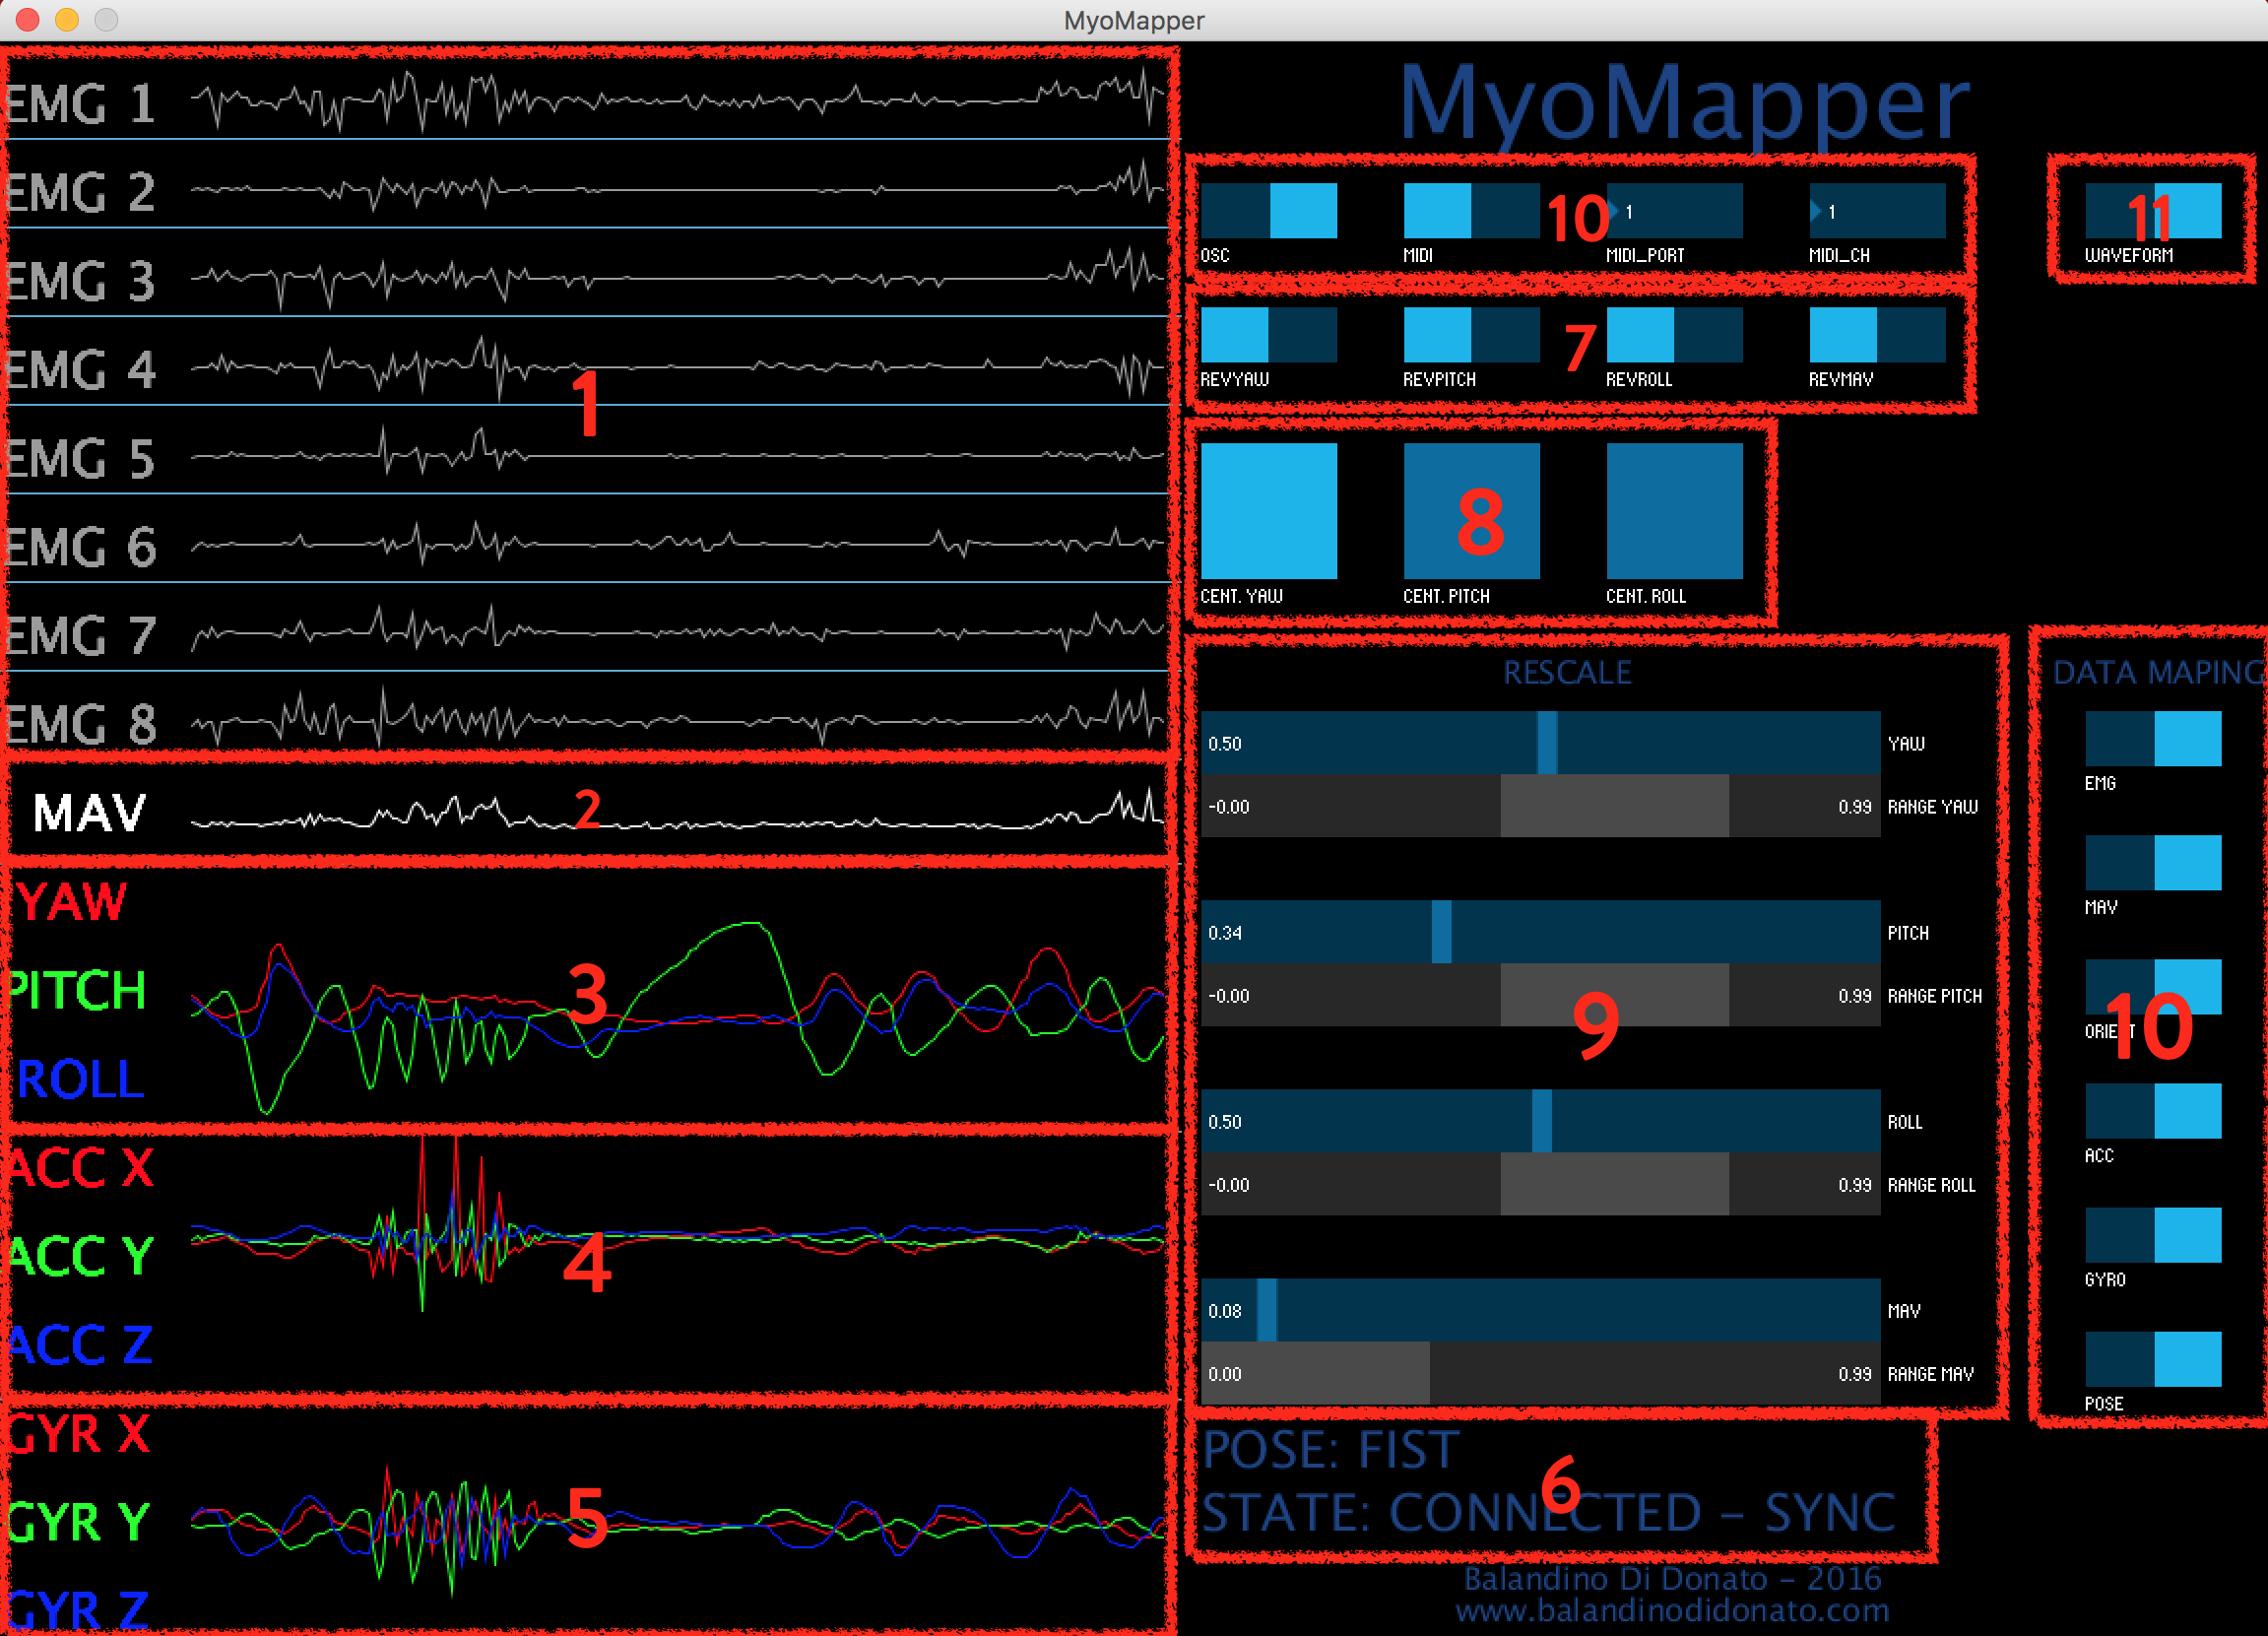
\includegraphics[width=1\linewidth]{../MyoMapper}
		\caption{Myo Mapper screenshot}
		\label{fig:MyoMapperGUI}
	\end{figure}
	
		\subsection{Myo data visualisation}
		The Myo data visualisation can be enabled or disabled by the toggle on the top right of the window. By disabling the Myo data visual representation you can save CPU, which in some cases may be useful for other process.
		
			\begin{figure}[h]
				\centering
				
\includegraphics[width=0.1\linewidth]{../MyoMapper-Waveform}
				\caption{Visual representation toggle}
				\label{fig:MyoMapper-Waveform}
			\end{figure}

		\subsection{EMGs}
		The first portion of graph on the left side desctibes the 8 EMG signals.
		
			\begin{figure}[h]
				\centering
				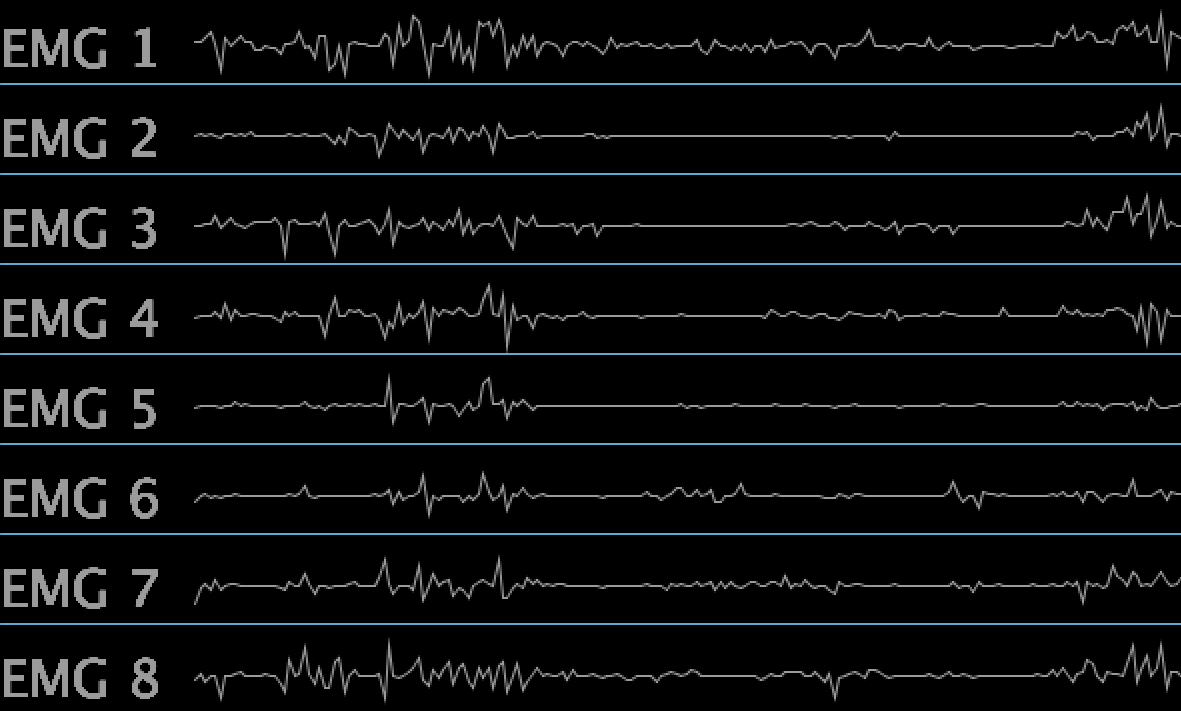
\includegraphics[width=0.6\linewidth]{../MyoMapper-EMG}
				\caption{Visual representation toggle}
				\label{fig:MyoMapper-EMG}
			\end{figure}
		
		EMG signals have been numbered following the enumeration by Thalmic Lab\footnote{EMG pad enumeration, \url{https://developer.thalmic.com/forums/topic/255/}}.
		
		\begin{figure}[h]
			\centering
			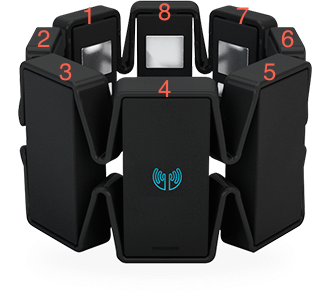
\includegraphics[width=0.4\linewidth]{../EMG-myo-pad-enumeration}
		    \caption{Source immage: Arief, Z., Sulistijono, I. A., \& Ardiansyah, R. A. (2015) Comparison of five time series EMG features extractions using Myo Armband. \textit{International Electronics Symposium (IES)},  (pp. 11-14). IEEE. Chicago.}
			\label{fig:EMG-myo-pad-enumeration}
		\end{figure}
		
		\subsection{MAV}

		MAV stand for Mean Absolute Value, which in this case refers to the EMGs' MAV. In Myo Mapper the EMG's MAV is calculated through the following formula from (Arief et al. 2015)\footnote{Arief Z., Sulistijono I. A., Ardiansyah R. (2015) A. Comparison of five time series EMG features extractions using Myo Armband, \textit{International Electronics Symposium (IES)}, 11 - 14, Surabaya.}.
		
		\begin{math}
		     MAV = \dfrac{1}{N} \displaystyle\sum_{k-1}^{N} \lvert X_{k} \rvert
		\end{math}
		
				\begin{figure}[h]
					\centering
					
\includegraphics[width=0.6\linewidth]{../MyoMapper-MAV}
					\caption{Mean Absolute Value (MAV)}
					\label{fig:MyoMapper-MAV}
				\end{figure}
	
		\subsection{Orientation}
		The orientation data: yaw, pitch and roll are displayed in a merged graph, and they appear respectively in green, red and blue.
		
		\begin{figure}[h]
			\centering
			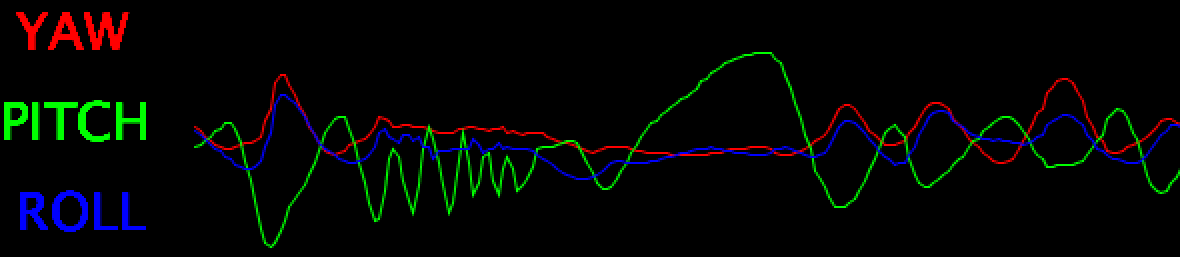
\includegraphics[width=0.6\linewidth]{../MyoMapper-YPR}
			\caption{Orientation data}
			\label{fig:MyoMapper-Orientation}
		\end{figure}
	
		\subsection{Acceleration}
		The acceleration data have been represented following the same method adopted for the orientation data. Here, acceleration \textit{x}, \textit{y} and \textit{z} are respectively red, green and blue.
	
		\begin{figure}[h]
			\centering
			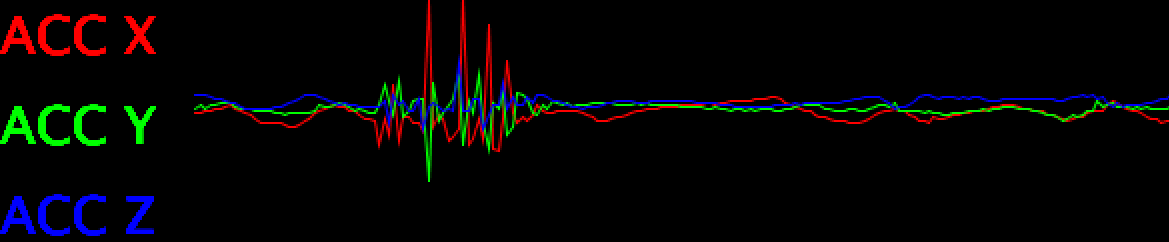
\includegraphics[width=0.6\linewidth]{../MyoMapper-Acc}
			\caption{Acceleration data}
			\label{fig:MyoMapper-Acc}
		\end{figure}	
		
		\subsection{Gyro}
		As for the acceleration data the gyro data have been represented following the same method adopted for the orientation data. Here, gyro \textit{x}, \textit{y} and \textit{z} are respectively red, green and blue.
		
		\begin{figure}[h]
			\centering
			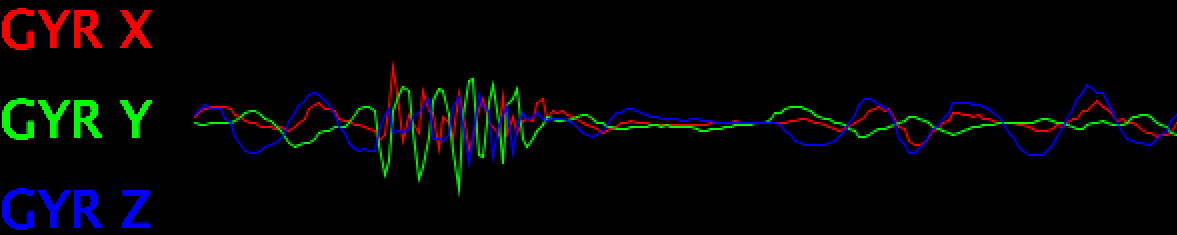
\includegraphics[width=0.6\linewidth]{../MyoMapper-Gyro}
			\caption{Gyro data}
			\label{fig:MyoMapper-Gyro}
		\end{figure}	
		
		\subsection{OSC and MIDI control}

		On the right side of the Myo Mapper, all controls to manage the Myo's data.
		
		The first line of controls is composed by a OSC and MIDI toggle to respectively allow or not Myo Mapper to send OSC and MIDI messages to third applications. The number boxes next to the MIDI toggle are to set up the MIDI port and channel (Fig. \ref{fig:MyoMapper-OSC-MIDI}).

		Moreover, it is possible to select the data to send to the third application by enabling or disabling respective the toggles on the right side (Fig. \ref{fig:MyoMapper-DataMapping}).
		
		\begin{figure}[h]
			\centering
			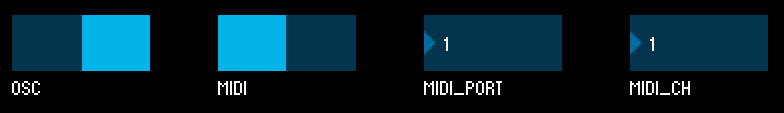
\includegraphics[width=0.6\linewidth]{../MyoMapper-OSC-MIDI}
			\caption{OSC and MIDI control}
			\label{fig:MyoMapper-OSC-MIDI}
		\end{figure}
		
		\begin{figure}[h]
			\centering
			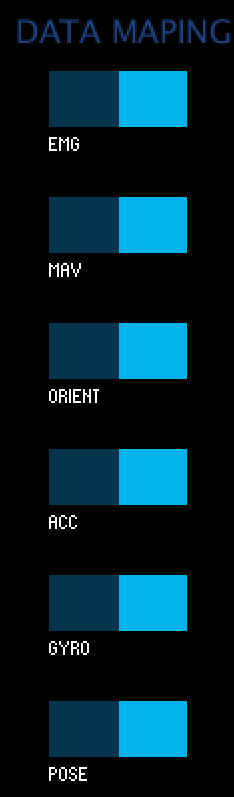
\includegraphics[height=0.6\linewidth]{../MyoMapper-DataMapping}
			\caption{OSC and MIDI data mapping}
			\label{fig:MyoMapper-DataMapping}
		\end{figure}
		
		\subsection{Myo data elaboration}
		Myo data reference point, specifically the Yaw data is established once the Myo is turned on. Thus, incoming Myo data may be different despite orienting the Myo in the same position. Moreover, it has been experienced by many Myo users a data drift of the yaw parameter.
		For this reasons, in Myo Mapper are implemented a functions to reverse, rescale and centre Myo data.
		
		\subsubsection*{Reverse Data} 
		Reverse data toggles allow the user to reverse the yaw, pitch, roll and MAV value.
		
		\begin{figure}[h]
			\centering
			
\includegraphics[width=0.6\linewidth]{../MyoMapper-Rev}
			\caption{Reverse}
			\label{fig:MyoMapper-Rev}
		\end{figure}		

		\subsubsection*{Centre Data}
		Centre data bangs allow to set the current yaw, pitch, roll values at 0.5 and so rescaling the data accordingly.
		
		\begin{figure}[h]
			\centering
			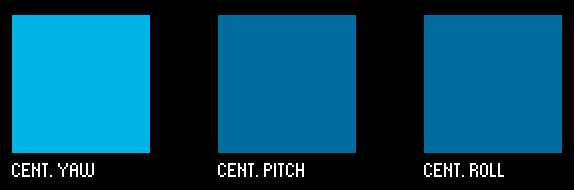
\includegraphics[width=0.6\linewidth]{../MyoMapper-Centr}
			\caption{Centre data}
			\label{fig:MyoMapper-Centr}
		\end{figure}		
		
		\subsubsection*{Rescale Data}
		Rescale data sliders, grey and are placed just under a blue sliders, which function is to monitor the data (Fig. \ref{fig:MyoMapper-Rescale}).  Rescale data sliders allow to rescale the Myo data within a certain range. It is possible to set a minimum value with the left edge of the slider, the maximum with the right edge and the whole range can be transposed by moving the slider from its centre.
		
		\begin{figure}[h]
			\centering
			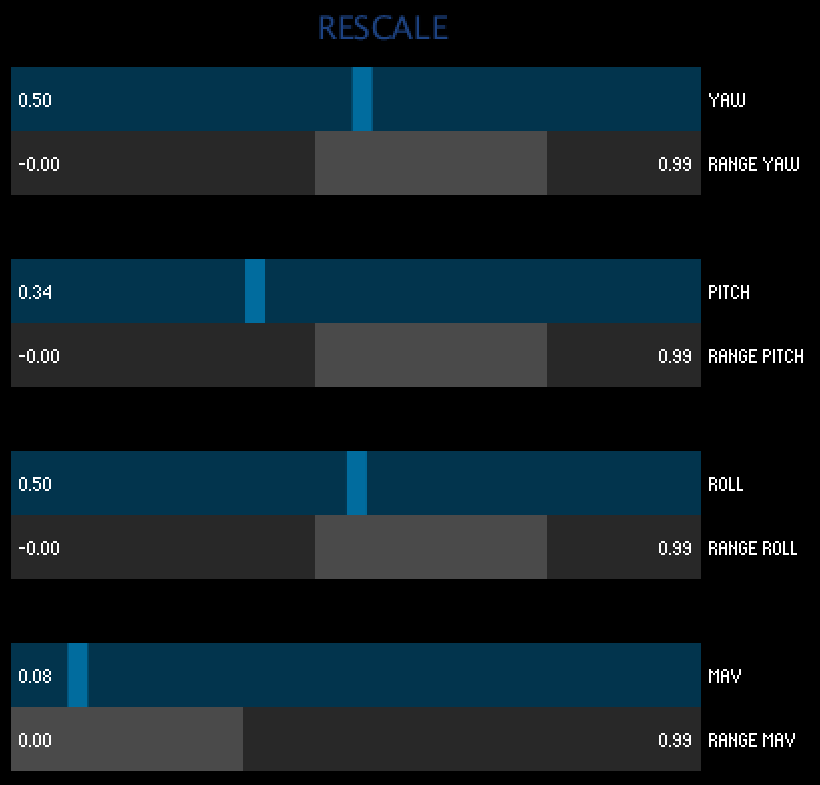
\includegraphics[width=0.6\linewidth]{../MyoMapper-Rescale}
			\caption{Rescale data}
			\label{fig:MyoMapper-Rescale}
		\end{figure}
	
	\subsection{Pose and Myo status}
	The recognised hand posed and the status are displayed by two labels underneath the rescale data sliders.
	
	\begin{figure}[h]
		\centering
		
\includegraphics[width=0.6\linewidth]{../MyoMapper-Pose-Status}
		\caption{Pose and Myo status}
		\label{fig:MyoMapper-Pose-Status}
	\end{figure}	
		 
\newpage
\section{OSC and MIDI}
	\subsection{OSC connection}
	
	Myo Mapper sends OSC messages at the port number 5432. To change it:
	
	\begin{itemize}
	\item  Open the osc.pde file within the MyoMapper folder
		\begin{verbatim}
		open <path>/<to>/MyoMapper/MyoMapper/osc.pde
		\end{verbatim}
	\item Edit the number port (latest number) at the 10th code line
		\begin{verbatim}
	    myRemoteLocation = new NetAddress("127.0.0.1",5432);
	    \end{verbatim}
	\item Save the osc.pde file
	\item Build Myo Mapper or compile it from Processing.
    \end{itemize}
	\subsection{OSC Mapping}
	
	\begin{tabular}{|c|c|c|c|}\hline
		\textbf{Myo parameter}   & \textbf{OSC tag} & \textbf{n. values} & \textbf{Range Values} \\ \hline
		EMG 1, EMG 2, ..., EMG 8 &  /emg        & 8         &  -128 , 127  \\ \hline
		MAV                      & /emgMav      & 1         & 0. , 1.      \\\hline 
		Yaw, Pitch, Roll         & /orientation	& 3         & 0. , 1.      \\ \hline
		Acc X, Y, Z              & /acc         & 3         & 0 , 1000     \\ \hline
		Gyro X, Y, Z             & /gyro        & 3         & 0. , 2PI     \\ \hline
		Pose                     & Pose         & 2         & "pose", 0 - 5 \\ \hline
	\end{tabular} \\ \ \\
	
	Following the hand pose mapping.
	
	\begin{tabular}{|c|c|c|}\hline
		\textbf{Pose}  & \textbf{String} & \textbf{Int} \\ \hline
		Rest           & REST            & 0 \\ \hline
		Fist           & FIST            & 1 \\ \hline
		Fingers Spread & FINGERS\_SPREAD  & 2 \\ \hline
		Wave In        & WAVE\_IN         & 3 \\ \hline
		Wave Out       & WAVE\_OUT        & 4 \\ \hline
		Double Tap     & DOUBLE\_TAP      & 5 \\ \hline
	\end{tabular}  
	
	\subsection{MIDI connection}
	
	The MIDI port can be changed through the user interface once you have built the application. In order to change MIDI channel to which send MIDI data it is also doable through the GUI. To change cc value of the single Myo value, you need to open the relative pde file and edit the parameters of the functions which send MIDI data. For Example, to change cc values relative to Myo acceleration values you have to open the myoAcceleration.pde file
	\begin{verbatim}
		open <path>/<to>/MyoMapper/MyoMapper/myoAcceleration.pde
	\end{verbatim}	

	Then, edit the function to send MIDI data.
	\begin{verbatim}
		myBus.sendControllerChange(chMIDI, 4, rollMIDI);
	\end{verbatim}
	
	where \textit{chMIDI} is the midi channel, \textit{4} is the cc value and \textit{rollMIDI} is the velocity value.
	
	\subsection{MIDI mapping}
	\begin{tabular}{|c|c|c|}\hline
		\textbf{Myo parameter} & \textbf{cc value} & \textbf{Velocity} \\ \hline
		EMG1 & 1 & 0, 127 \\ \hline
		EMG2 & 2 & 0, 127 \\ \hline
		EMG3 & 3 & 0, 127 \\ \hline
		EMG4 & 4 & 0, 127 \\ \hline
		EMG5 & 5 & 0, 127 \\ \hline
		EMG6 & 6 & 0, 127 \\ \hline
		EMG7 & 7 & 0, 127 \\ \hline
		EMG8 & 8 & 0, 127 \\ \hline
		MAV  & 9 & 0, 127 \\ \hline
		Yaw & 10 & 0, 127 \\ \hline
		Pitch & 11 & 0, 127 \\ \hline
		Roll & 12 & 0, 127 \\ \hline
		Acc X & 13 & 0, 127 \\ \hline
		Acc X & 14 & 0, 127 \\ \hline
		Acc X & 15 & 0, 127 \\ \hline
		Gyro X & 16 & 0, 127 \\ \hline
		Gyro X & 17 & 0, 127 \\ \hline
		Gyro X & 18 & 0, 127 \\ \hline
		Pose: Rest & 19  & 0 \\ \hline
		Pose: Fist & 19 & 25 \\ \hline
		Pose: Fingers Spread & 19 & 50 \\ \hline
		Pose: Wave In & 19 & 76 \\ \hline
		Pose: Wave Out & 19 & 101 \\ \hline
		Pose: Double Tap & 19 & 127 \\ \hline
	\end{tabular} 
\newpage	
\section{Build Myo Mapper}
\begin{enumerate}
	\item Download:
	\begin{itemize}
		\item Processing 2.2.1\footnote{Processing, \url{https://processing.org/download/}}
		\item Libraries for Processing:
		\subitem - The midibus\footnote{midibus, \url{http://www.smallbutdigital.com/themidibus.php}}
		\subitem - ControlP5\footnote{ControlP5, \url{http://www.sojamo.de/libraries/controlP5/}}
		\subitem - oscP5\footnote{oscP5, \url{http://www.sojamo.de/libraries/oscP5/}}
		\subitem - Myo For Processing\footnote{Myo for Processing, \url{https://github.com/nok/myo-processing}}
	\end{itemize}
	\item Create a folder called Myo Mapper
	\item Open a Terminal and change your directory to the Myo Mapper Folder
	\begin{verbatim} cd <path>/<to>/MyoMapper \end{verbatim}
	\item Clone the repository
	\begin{verbatim} git clone https://github.com/balandinodidonato/MyoMapper \end{verbatim}
	\item Open the MyoMapper.pde file
	\item open MyoMaper/MyoMapper.pde
	\item Navigate to the top bar and select:
	\subitem - File
	\subitem - Export Application 
	\item Select the Platform which you will be working on
	\item Click on Export
\end{enumerate}

\newpage
\section{Interactive performance with Myo and Myo Mapper}

Myo Mapper is a software which enable the user to drive audio and visual elaborations, within third software able to receive OSC  and MIDI messages, using the Myo armband.

To get started with your interactive performance you can download examples for Integra Live\footnote{Integra Live, \url{http://integralive.org/}}, Pd\footnote{Pure Data (aka Pd), \url{https://puredata.info}} and Max\footnote{Max, \url{https://cycling74.com/products/max/}} trough the following link.

\url{http://www.balandinodidonato.com/myomapper/}

\end{document}